\documentclass{scrartcl}

%\usepackage{natbib}
\usepackage{latexrc/macros}

\addbibresource{biblio.bib}

\title{Metastability for the Contact Process on $\integer$}
\author{Owen Lynch \and Kacper Urbański}
\DeclareMathOperator{\expDist}{Exp}
\newcommand{\ep}{\varepsilon}
\begin{document}

\maketitle
\begin{abstract}
    Metastability is the coexistence of an equilibrium and a ``quasi-equilibrium'' (metastable) state in a system. If we look at a metastable system in time domain, it 
    initially appears to have stabilized in the ``quasi-equilibrium'' state,
    until it suddenly relaxes to the true equilibrium. Metastability is a common phenomenon in nature, with examples ranging from physics to economics and social sciences. 
    This work is a summary of a paper by R. Schonmann \cite{schonmann}, which
    frames this phenomenon as a rigorous property of an abstract interacting particle system - the Contact Process.
\end{abstract}

\section{Overview - what's metastability?} \label{overview}

Take a family of Markov processes $\{\xi_N(t)\}_{N\in\mathbb{N}}$. The essential idea behind metastability is that, if we were to discretize (``coarse-grain'') time, increasing $N$
would make
the process under consideration look more and more like the Markov process in \fref{fig:metastability_nutshell}.

\begin{figure}[h!]
  \centering
  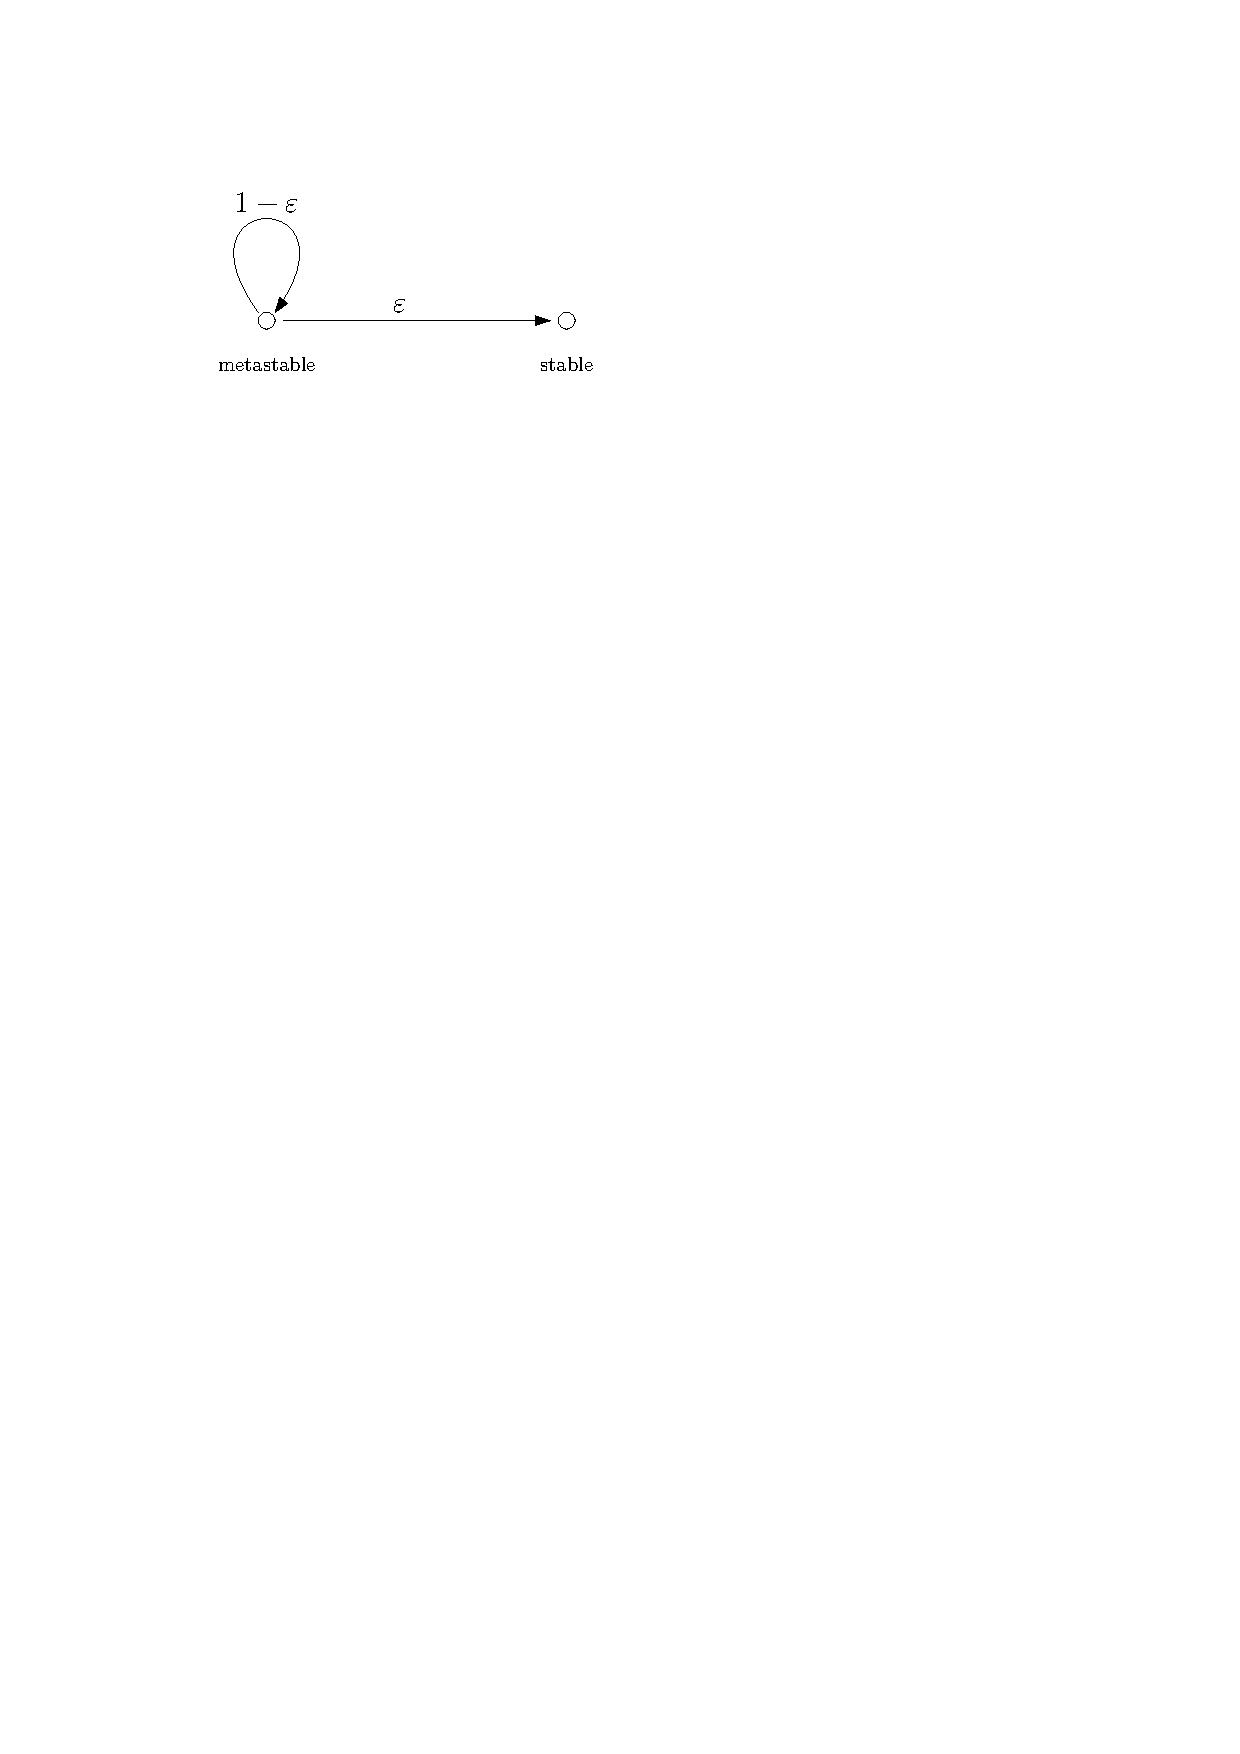
\includegraphics{presentation_owen/metastable_coarse_grain.pdf}
  \caption{Metastability in a Nutshell}
  \label{fig:metastability_nutshell}
\end{figure}

In other words, the system begins in a so-called ``metastable state'', and has a very small chance to move to the stable state at any time. The stable state is either absorbing, or close-to absorbing; in the case that we will talk about in this paper, the stable state is absorbing.

In order to make this ``coarse-graining'' happen, we need two things to be true asymptotically.

\begin{enumerate}
  \item The hitting time of the stable state is exponentially distributed.
  \item Up until the hitting time, temporal means of measurements made to the process converge to an expectation of those measurements with respect to some stationary distribution.
\end{enumerate}

Together, these two properties intuitively allow us to approximate the entire process by sampling from the stationary distribution up until the hitting time, and then putting the system in the absorbing state.

The difficulty comes in stating these two properties precisely. To do this, suppose that $T_{N}$ is the hitting time of the absorbing state, $\mu$ is the stationary distribution, 
and $R_{N}$ is a ``time scale'' parameter that satisfies $R_{N}/\E T_{N} \to 0$. Then we rewrite the two properties more formally as

\begin{enumerate}
  \item $T_{N} / \E T_{N} \to \expDist(1)$ in distribution as $N \to \infty$.
  \item For any $f$ cylindrical,
    \[ \int_{S}^{S + R_{N}} f(\xi_{N}(t)) dt \to \mu(f) \]
    as $N \to \infty$, for any $S + R_{N} < T_{N}$.
\end{enumerate}

This second statement is still very imprecise, and actually mathematically meaningless as currently posed. Also, it turns out that we want a much stronger statement than that. However, we hope that this first statement should ``innoculate'' the reader to the precise statement, which is fairly dense on its own.

\section{Review of Contact Process}

\subsection{Basic Definitions}
% TODO Proposition: remove this fragment to free up space
%The contact process on $\integer$ can be defined by the Markov pregenerator $L$ with domain cylindrical functions $2^{\integer} \to \real$ given by
%\begin{equation}
%  \label{eq:contact_generator}
%  Lf(\eta) = \sum_{x \in \integer} c(x,\eta) (f(\eta^{x}) - f(\eta))
%\end{equation}
%where
%\begin{equation*}
%  c(x,\eta) = \begin{cases}
%    1 & \qif* \eta(x) = 1 \\
%    \lambda(\eta(x-1) + \eta(x+1)) & \qif* \eta(x) = 0
%  \end{cases}
%\end{equation*}
%$\lambda$ is the single parameter for the contact process; we will discuss this more later.

We could succinctly define the Contact Process by using its Markov generator. However, for our purposes we will use
an alternative definition that lends itself better to certain constructions that are useful in proofs concerning metastability.

First we construct a ``percolation structure'', which consists of for each $x \in \integer$
\begin{enumerate}
  \item A Poisson process $P_{x}$ with rate 1, which we call the ``death'' process at $x$.
  \item A Poisson process $P_{x \to x+1}$ with rate $\lambda$, which we call the ``right infection'' process at $x$.
  \item A Poisson process $P_{x \to x-1}$ with rate $\lambda$, which we call the ``left infection'' process at $x$.
\end{enumerate}

We consider $P_{x}$ to be a random element of $\powerset(\real)$, i.e. $t \in P_{x}$ if and only if the Poisson process ``ticks'' at time $t$.

%\begin{figure}[h!]
%  \centering
%  % TODO
%  \caption{Example Percolation Structure}
%  \label{fig:ex_perc_structure}
%\end{figure}

We define a ``path'' between $(x,s), (y,t) \in \integer \by \real$ with $s \leq t$ to be a sequence
$(z_{0},r_{0}), \ldots, (z_{n},r_{n})$ with $r_{i} \leq r_{i+1}$ such that for all $(z_{i},r_{i}),(z_{i+1},r_{i+1})$, either
\begin{enumerate}
  \item $r_{i} = r_{i+1}$, $\abs{z_{i} - z_{i+1}} = 1$, and $r_{i} \in P_{z_{i} \to z_{i+1}}$. In this case, we are jumping laterally by one line at a time of infection.
  \item $z_{i} = z_{i+1}$, and $[r_{i},r_{i+1}] \cap P_{z_{i}} = \emptyset$. In this case, we are moving along a vertical line, uninterrupted by any deaths.
\end{enumerate}

Define $\xi^{A}(t)$ to be the set of $y$ such that there is a path from $(x,0)$ to $(y,t)$ for some $x \in A$. If the superscript is omitted, then we assume $A = \integer$, i.e. $\xi(t) = \xi^{\integer}(t)$.

For any $A \ins B$, we define $\xi_{B}^{A}(t)$ to be the set of $y$ such that there is a path from $(x,0)$ to $(y,t)$ for some $x \in A$ that stays entirely within $B$. As a special case, we let $\xi_{N}^{A}(t) = \xi_{[-N,N]}^{A}$, for $N \in \natural$. Note that $\xi_{B}$ takes values exclusively in $\powerset(B)$.

\subsection{Useful Properties} \label{useful_properties}

One of the most important facts about the contact process is that there is a critical value of $\lambda$, $\lambda_{c}$. For $\lambda < \lambda_{c}$, $\xi(t)$ has a unique 
extremal invariant measure $\delta_{\emptyset}$. At $\lambda = \lambda_{c}$ the system undergoes a phase transition - for $\lambda > \lambda_{c}$, another extremal invariant 
measure $\mu$ appears, with the property that
\[ \mu(f) = \limas_{T \to \infty} \frac{1}{T} \int_{0}^{T} \E f(\xi(t)) \dd{t} \]
This measure is not concentrated at $\emptyset$.

For $\xi_{N}(t)$, the only invariant measure is $\delta_{\emptyset}$, because $\emptyset$ is a trap and $\xi_{N}$ takes values on a finite state space. 
However, as mentioned before, for $\lambda > \lambda_{c}$ an analogue of a phase transition takes place. The system starts being metastable, and stays distributed
\emph{approximately} as $\mu$, before a sudden fluctuation takes it to $\emptyset$.

%TODO: Proposition: remove this to make space
%TODO: give brief explanations for each of these.
%
%\begin{proposition}
%$\Prob(\xi(t) \cap A \neq \emptyset)$ monotonically decreases to $\mu(\eta \st \eta \cap A \neq \emptyset)$.
%\end{proposition}
%
%\begin{proposition}
%The contact process is \emph{self-dual}.
%\end{proposition}
%
%\begin{corollary}
%$\Prob(\xi^{A}(s) \neq \emptyset, \forall s \geq 0) = \mu(\eta \st \eta \cap A \neq \emptyset)$
%\end{corollary}
%
%\begin{proposition}
%Let $\rho = \Prob(\xi^{\set{0}}(s) \neq \emptyset) = \mu(\eta \st \eta(0) = 1)$, if $\lambda$ is the parameter for $\xi$. Then if $\lambda > \lambda_{c}$ then $\rho > 0$. This will later be an important quantity for proofs.
%\end{proposition}
%
%\begin{proposition}
%$\mu$ is translation-invariant, and even better, ergodic under translations. This means that one can approximate $\mu(f)$ by averaging $\E \tau_{i}f(\xi(t))$ over a large number of $i$, where $\tau_{i}f(\eta)$ is $f$ applied to $\eta$ shifted by $i$. Finally, $\mu$ has exponentially decaying correlations; that is if $\set{X_{i}}_{i \in \integer}$ is distributed according to $\mu$, then the correlation between $X_{i}$ and $X_{j}$ decays exponentially with $\abs{i - j}$.
%\end{proposition}

%TODO Proposition: reduce this section take up 1.75 of the page max. I do the same for Theorem 2
\section{Hitting Time of Stable State}

\begin{theorem}[from \cite{schonmann}]
  If $T_{N} = \inf\set{t > 0 \st \xi_{N}(t) \neq \emptyset}$, then
  \[ \frac{T_{N}}{\E T_{N}} \to \expDist(1) \]
  in distribution.
\end{theorem}

Without further ado, we get down to the proof. First of all, we replace $\E T_{N}$ by the unique (by monotonicity) $\beta_{N}$ such that $\Prob(T_{N} > \beta_{N}) = \e^{-1}$. At the end, we will show that $\frac{\E T_{N}}{\beta_{N}} \to 1$.

Now let $G_{N}(t) = \Prob[\frac{T_{N}}{\beta_{N}} > t]$, the CDF of $T_{N}/\beta_{N}$. Similarly, let $G_{N}^{A}(t) = \Prob[\frac{T^{A}_{N}}{\beta_{N}} > t]$. Note that $G_{N}^{A}(t) \leq G_{N}(t)$ To show that $T_{N}/\beta_{N}$ converges in distribution to $\expDist(1)$, we must show that $G_{N}(t) \to \e^{-t}$. This can be accomplished by showing that
\[ \limas_{N \to \infty} \abs{G_{N}(t+s) - G_{N}(t)G_{N}(s)} = 0 \]
for all $t,s > 0$.

%Note that $G_{N}(t) = \Prob[\xi_{N}(t) \neq \emptyset]$, as $\xi_{N}$ is ``alive'' at time $t$ if and only if $T_{N} > t$. Thus,
%
%\begin{align*}
%  G_{N}(t+s) &= \Prob[\xi_{N}(t+s) \neq \emptyset] \\
%             &= \sum_{A \neq \emptyset} \Prob[\xi_{N}(t+s) \neq \emptyset | \xi_{N}(t) = A] \Prob[\xi_{N}(t) = A] \\
%             &= \sum_{A \neq \emptyset} G_{N}^{A}(s) \Prob[\xi_{N}(t) = A] \\
%             &\leq G_{N}(s) \sum_{A \neq \emptyset} \Prob[\xi_{N}(t) = A] \\
%             &= G_{N}(s) G_{N}(t)
%\end{align*}
%
%Therefore, we are looking to show that $G_{N}(s) G_{N}(t) - G_{N}(t+s) \to 0$ (we can forget the absolute value signs).

It is at this point that we introduce a curious little construction, which seems to not make much sense at first but turns out to be the key to the entire proof. Define $F_{b}$ for $b > 0$ by

\[ F_{b} = \left\{A \ins \integer \st \frac{\abs{A \cap [-b,-1]}}{b} > \frac{\rho}{2}, \frac{\abs{A \cap [1,b]}}{b} > \frac{\rho}{2}\right\} \]

%Recall that $\rho$ was defined in \ref{prop:rho_lambda} to be the probability that $\xi^{\set{0}}$ never dies. The intuition that the reader should hold for $F_{b}$ is that it is the set of $A$ that are ``sufficiently dense'' on $[-b,-1]$ and $[1,b]$ so that $\xi^{A}_{N}$ behaves just like $\xi_{N}$. The reason we have this ``two-sided'' condition is that we will use the processes $\xi_{(-\infty,N)}$ and $\xi_{(-N,\infty)}$, which have invariant measure $\mu$ as well, to talk about $\xi_{N}$.

For $A \in F_b$ we have
\begin{align*}
  %G_{N}(t+s) &= \sum_{A \neq \emptyset} G_{N}^{A}(t) \Prob[\xi_{N}(\beta_{N}s) = A] \\
  %&\geq \sum_{A \in F_{b}} G_{N}^{A}(t) \Prob[\xi_{N}(\beta_{N}s) = A] \\
  %&\geq \min_{A \in F_{b}} G_{N}^{A}(t) \Prob[\xi_{N}(\beta_{N}s) \in F_{b}]
  G_{N}(t+s)
  \geq \min_{A \in F_{b}} G_{N}^{A}(t) \Prob[\xi_{N}(\beta_{N}s) \in F_{b}]
\end{align*}
(We assume that $A \ins [-N,N]$ when such an assumption is necessary).

After some simple algebra we get the following bound:
\begin{align*}
  G_{N}(t)G_{N}(s) - G_{N}(t+s) \leq& G_{N}(t) - \min_{A \in F_{b}} \Prob[\xi_{N}^{A}(\beta_{N}t) \neq \emptyset]+ \Prob[\xi_{N}(\beta_{N}s) \neq \emptyset, \xi_{N}(\beta_{N}s) \notin F_{b}]
\end{align*}
%\begin{align*}
%  G_{N}(t)G_{N}(s) - G_{N}(t+s) \leq& \; G_{N}(t)G_{N}(s) - \min_{A \in F_{b}} G_{N}^{A}(t) \Prob[\xi_{N}(\beta_{N}s) \in F_{b}] \\
%  =& \; G_{N}(s)(G_{N}(t) - \min_{A \in F_{b}} G_{N}^{A}(t)) \\
%                                 &+ \min_{A \in F_{b}} G_{N}^{A}(t)(G_{N}(s) - \Prob[\xi(\beta_{N}s) \in F_{b}]) \\
%  \leq& \; (G_{N}(t) - \min_{A \in F_{b}} \Prob[\xi_{N}^{A}(\beta_{N}t) \neq \emptyset]) \\
%                                 &+ \Prob[\xi_{N}(\beta_{N}s) \neq \emptyset, \xi_{N}(\beta_{N}s) \notin F_{b}]
%\end{align*}

We will have finished if for any $\ep > 0$, we can find $b(\ep)$ and $N(\ep) > b(\ep)$  such that for $N \geq N(\ep)$ and $A \in F_{b}$, we have both
\begin{align}
  G_{N}(t) - G_{N}^{A}(t) &< \ep \label{eq:firstineq} \\
  \Prob[\xi_{N}(\beta_{N}s) \neq \emptyset, \xi_{N}(\beta_{N}s) \notin F_{b}] &< \ep \label{eq:secondineq}
\end{align}

We tackle \eref{eq:firstineq} first. Remember that $\xi_{N}(t)$ and $\xi_{N}^{A}$ are defined on the same percolation structure. Therefore, $\xi_{N}(t) \supset \xi_{N}^{A}(t)$, so we have
\[ \Prob[\xi_{N}(\beta_{N} t) \neq \emptyset] - \Prob[\xi_{N}(\beta_{N} t) \neq \emptyset] = \Prob[\xi_{N}(\beta_{N} t) \neq \emptyset, \xi_{N}^{A}(\beta_{N} t) = \emptyset] \leq \Prob[T_{N} \neq T_{N}^{A}] \]
%The intuition for why the right hand side of this is small is that once $\xi_{N}(t_{0}) = \xi_{N}^{A}(t_{0})$, then for all $t > t_{0}$, $\xi_{N}(t) = \xi_{N}^{A}(t)$. Therefore, as long as the event $\xi_{N}(t_{0}) = \xi_{N}^{A}(t_{0})$ happens before $T_{N}^{A}$, we will have $T_{N}^{A} = T_{N}$. Let $E$ be this event; we must show that $\Prob(E) > 1 - \ep$.
%

Set $E = \{T^A_N = T_N\}$. As $\lambda > \lambda_{c}$, we can find $n(\ep)$ such that
\[ \mu(B \st B \cap [1,n(\ep)] = \emptyset) \leq \frac{\ep}{2} \]

Then take $b = b(\ep)$ such that $n(\ep) \leq b \cdot \rho/2$. For $A \in F_{b}$, $\abs{A \cap [-b,-1]} \geq b \cdot \rho/2 \geq n(\ep)$, so
\[ \Prob[T_{[-N,\infty)}^{A \cap [-b,-1]} = \infty] \geq \Prob[T_{[-N,\infty]}^{[-N,\ldots,-N+n(\ep)]} = \infty] \geq 1 - \frac{\ep}{2} \]
First inequality follows from the fact that $A \cap [-b,-1]$ is at least as spread out as $[-N,\ldots,-N+n(\ep)]$. A process which is more spread out has more chances of infecting 
healthy individuals, and so survives longer.
The second inequality follows from duality and monotone convergence.

Similarly, $\Prob[T_{(-\infty,N]}^{A \cap [1,b]} = \infty] \geq 1 - \frac{\ep}{2}$. Let $E'$ be the event that both of these stopping times are infinite; clearly $P(E') \geq 1 - \ep$. It remains to show that $E \supset E'$.

Define stopping times
\begin{align*}
  U &= \inf\set{t > 0 \st N \in \xi_{[-N,\infty)}^{A \cap [-b,-1]}(t)} \\
  V &= \inf\set{t > 0 \st -N \in \xi_{(-\infty,N]}^{A \cap [1,b]}(t)}
\end{align*}
Until $U$, $\xi_{N}^{A \cap [-b,-1]}(t) = \xi_{[-N,\infty)}^{A \cap [-b,-1]}(t)$. Therefore, on $E'$, $\xi_{N}^{A \cap [-b,-1]}(t)$ is alive up until $U$, whence $\xi_{N}^{A}$ is alive up until $U$. Similarly, $\xi_{N}^{A}$ is alive up until $V$. Therefore, on $E'$, $T_{N} \geq T_{N}^{A} > \max(U,V)$.

However, for $t > \max(U,V)$, I claim that $\xi_{N}(t) = \xi_{N}^{A}(t)$. To see this, any path to $x \in \xi_{N}(t)$ must either cross the path that goes from $A \cap [-b,-1]$ at time $0$ to $N$ at time $U$ or the path that goes from $A \cap [1,b]$ at time $0$ to $-N$ at time $V$. Therefore, there is a path from $A$ at time $0$ to $x$ at time $t$, whence $x \in \xi_{N}^{A}(t)$. Therefore, on $E'$, $T_{N} = T_{N}^{A}$, and we have shown \eref{eq:firstineq}.

Equation~\ref{eq:secondineq} also relies crucially on the percolation structure. Let $D_{b} = F_{b}^{C} \setminus \set{\emptyset}$. Then we must show that $\Prob(\xi_{N}(\beta_{N}s) \in D_{b}) < \ep$. To do this, note that as long as $\xi_{N}(t)$ is alive, we have
\[ \xi_{N}(t) = \xi(t) \cap [\min \xi_{N}(t), \max \xi_{N}(t)] \]
This is because any path to $x \in \xi(t) \cap [\min \xi_{N}(t), \max_{N}(t)]$ must either stay inside $[\min \xi_{N}(t), \max_{N}(t)]$, in which case $x \in \xi_{N}(t)$, or pass through the path to $\min \xi_{N}(t)$ or $\max \xi_{N}(t)$, in which case we also have $x \in \xi_{N}(t)$.

Therefore, as long as $\min \xi_{N}(\beta_{N}s) < -N + L$, $\max \xi_{N}(\beta_{N}s) > N - L$ and $\xi_{N}(\beta_{N}s) \neq \emptyset$, we have $\xi(\beta_{N}s) \in D_{b}$ iff $\xi_{N}(\beta_{N}s) \in D_{b}$.

We can minimize $\xi(\beta_{N}s) \in D_{b}$ by picking $b > b''(\ep)$ sufficiently large. In order to use this, we use the following decomposition
\begin{align*}
  \Prob[\xi_{N}(\beta_{N}s) \in D_{b}] \leq&\; \Prob[\xi_{N}(\beta_{N}s) \in D_{b}, \min \xi_{N}(\beta_{N}s) < -N + L, \max \xi_{N}(\beta_{N}s) > N - L] \\
                                &+ \Prob[\min \xi_{N}(\beta_{N}s) \geq -N + L, \xi_{N}(\beta_{N}s) \neq \emptyset] \\
                                &+ \Prob[\max \xi_{N}(\beta_{N}s) \leq N - L, \xi_{N}(\beta_{N}s) \neq \emptyset]
\end{align*}
By what we noted earlier, the first term is less than $\Prob(\xi(\beta_{N}s) \in D_{b})$; pick $b$ such that this is less than $\frac{\ep}{3}$.

It remains to minimize the last two terms; by symmetry we only show how to minimize the first. Using a percolation structure argument, it is easy to show that as long as $\xi_{N}(\beta_{N}s) \neq \emptyset$, $\min \xi_{N}(t) = \min \xi_{[-N,\infty)}$. Therefore,
\begin{align*}
  \Prob[\min \xi_{N}(\beta_{N}s) \geq -N + L, \xi_{N}(\beta_{N}) \neq \emptyset] &\geq \Prob[\min \xi_{[-N,\infty)} \geq -N+L] \\
  &\geq \mu_{[-N,\infty)}\set{A \in [-N,\infty) \st A \cap [-N,-N+L-1] = \emptyset}
\end{align*}
Finally can pick $L$ large enough to make that last term less than $\frac{\ep}{3}$, and we have shown that everything can be made as small as we like, so we are done.

\section{Quasi-stationarity up to the Hitting Time}

Recall our initial description of Quasi-stationarity in Section \ref{overview}. To make it more precise, we will define 
\begin{itemize}
    \item \textbf{intermediate timescale} (for a given $N$) as $R_N \in \mathbb{R}_+$ with $R_N/\mathbb{E}[T_N] \rightarrow 0$
    \item \textbf{observable quantity} as a cylindrical (local) $f:\{0,1\}^\mathbb{Z} \rightarrow \mathbb{R}$
    \item \textbf{temporal mean} of observable quantity $f$ as
    \[
        A^N_{R_N}(s, f) := R_N^{-1}\int_s^{s+R_N}f(\xi_N(t))dt
    \]
    \item \textbf{fixed probability distribution} as $\mu$ (upper invariant measure of the Contact Process on $\mathbb{Z}$)
\end{itemize}
Note that $A^N_{R_N}$ is a random variable. We will say that this quantity \textbf{close} to $\mu(f)$ if the two converge in probabilty when $N \rightarrow \infty$.

It seems like the definitions given above would be sufficient to make our natural language definition of metastability formal. However, it turns out that an additional technical 
condition is needed. Define
    \[
        \Lambda(f) :=  \text{ smallest } B\subset \mathbb{Z} \text{ s.t. } f(A) = f(A\cap B) \ \forall A \subset \mathbb{Z}
    \]
    although this is not strictly true, we can think of $\Lambda(f)$ as the ``support'' of $f$.  

For our theorem to hold, we need to choose $L(\varepsilon, f) \in \mathbb{N}$, and we need to have that
\[
    L < N \text{~~and~~} \Lambda(f) \subset [-N+L, N-L]
\]
Notice that $L$ does not depend on $N$. Thus, since we chose to grow $N \rightarrow \infty$, having to choose this $L$ doesn't restrict our choice of $f$ - it merely sets the minimum
 $N$ we can consider.

 We're now ready to give a simplified formulation of what we mean by ``quasi-stationarity''
 \begin{theorem} [from \cite{schonmann}]
        If $\lambda > \lambda^*$ there is a sequence $\{R_N\}_{N \in \mathbb{N}} \subset \mathbb{R_+}$ such that:
        \begin{itemize}
            \item $R_N/\beta_N \rightarrow 0$ as $N\rightarrow \infty$
            \item For all $\varepsilon > 0$ and $f:\{0,1\}^\mathbb{Z} \rightarrow \mathbb{R}$ cylindrical,  $\exists L(\varepsilon, f) \in \mathbb{N}$ such that
                  \[
                      \mathbb{P}\left[ \max_{\mathbb{N}_0 \ni k < K_N}|A_{R_N}(kR_N, f) - \mu(f)| > \varepsilon\right] \rightarrow 0
                  \]
                  as $N \rightarrow \infty$, where $K_N = \max\{k \in \mathbb{N}_0: kR_N < T_N\}$ and $\Lambda(f) \subset [-N + L, N - L] \cap \mathbb{Z}$
        \end{itemize}
    \end{theorem}

Proof of this statement is beyond the scope of this article - we will merely give the reader some insight into its key points.

Central to all this business seems to be an issue of being able to make the exceedance probability (given below) arbitrarily small.
\[
    \mathbb{P}\left[ |A_{R_N}(kR_N, f) - \mu(f)| > \varepsilon\right]
\]
We ought to do so in a way which is uniform across all values of $K_N$ and $\mathbb{N}_0 \ni k < K_N$. We estimate this probabilty with a triangle inequality.
\footnotesize
\begin{equation}
    \mathbb{P}\left[ \left|R_N^{-1}\int_{kR_N}^{(k+1)R_N}f(\xi(t))dt - \mu(f)\right| > \varepsilon/2 \right] + 
    \mathbb{P}\left[ \left|R_N^{-1}\int_{kR_N}^{(k+1)R_N}f(\xi_N(t)) - f(\xi(t))dt \right| > \varepsilon/2\right]
    \label{th2:alternative}
\end{equation}
\normalsize
The first term can be made arbitrarily small, as a consequence of $\xi(t) \rightharpoonup \mu(f)$ and exponentially decaying temporal correlations of $\xi(t)$.

To shrink the second term in (\ref{th2:alternative}) we make extensive use of the graphical model construction of the Contact Process. We will say $\xi_N(t)$ is \textbf{wide} at $t$ if $\min\xi_N(t) < -N + L\ \land\ \max\xi_N(t) > N - L$.
By the fact that we construct all processes on the same percolation structure, and that interactions are between nearest neighbours, we have
\begin{lemma}[Shielding by a wide process]
    If $\xi_N(t)$ is wide at $t$, then \[\xi_N(t) = \xi(t)\text{ on }[-N + L, N - L] \cap \mathbb{Z}\]
    In particular, since $\Lambda(f) \subset [-N+L, N-L]$, we have $f(\xi_N(t)) = f(\xi(t))$
\end{lemma}
Thus, the second term of (\ref{th2:alternative}) will go to 0 if we're able to make it arbitrarily likely for $\xi_N$ to be wide. We can do so by setting $L$, but is it possible to do so such that its value is 
independent of $N$? 

Here we again make use of the percolation structure. Note that near $-N$, $\xi_N$ will ``look similar'' to $\xi_{[-N, +\infty)}$ (this is true as long as $\xi_N$ is alive). By the same reasoning, $\xi_N$ will ``look similar'' to $\xi_{(-\infty, N]}$ near $N$.
Hence we set $L$ such that
    \[
        \mu_{[-N, \infty)}\left( \left\{ A : A \cap [-N,-N+L] = \varnothing \right\} \right)  \leq \varepsilon/(16\norm{f})
    \]
This makes all possible states of $\xi_N$ that do not intersect $[-N, -N+L]$ very unlikely (by ``looking similar'' to $\xi_{[-N, \infty)}$). By symmetry, this also makes states
that do not intersect $[N-L, N]$ very unlikely. As a final stroke, we use translation invariance to notice that we will get exactly the same effect if we set $L$ 
    \[
        \mu_{[0, \infty)}\left( \left\{ A : A \cap [0,L] = \varnothing \right\} \right) \leq \varepsilon/(16\norm{f})
    \]
This concludes our overview of the proof of Theorem 2.

\printbibliography
        
\end{document}

